% Drawing 69/01-13 -- folder 69, batch 01, archive page 13 (PDF page 14).
% Transcription: en bas à gauche, une grille de droites croisées dont les cases portent $\alpha_4$, $\beta_4$, $\gamma_4$, $\alpha_1$, $\beta_2$, $\gamma_3$ et d'autres lettres, en partie illisibles
% Kind: grid of crossed lines with letters. Method 2 (schematic redraw from the facsimile). Status: partial.
% Notes: A grid of crossing straight lines: four steep lines falling to the right, three lines rising to the right and two nearly horizontal ones; each is drawn as one straight line, so the crossings are exact. The letters alpha_4, beta_4, gamma_4 (top row) and alpha_1, beta_2, gamma_3 (next row) are placed in their cells. Still differs from the facsimile: the lines are freehand and partly doubled on the page; the other letters in the cells (several 4s, overwritten indices) are left out, as the transcription calls them partly illegible. Redrawn 2026-11-09 (issue 128): vertices placed once and every edge drawn between them, labels at \small, strike-outs not drawn; to check again.
% Coordinates: 1 unit = 1 mm = 1/100 of the crop width (bbox in page fractions: [0.12, 0.75, 0.32, 0.83]).
% Redrawn by Claude (claude-opus-5-5), issue #73, 2026-11-09; not checked by a human; not compiled (no TeX in the session).
% Rights: reproduces part of the work -- behind RENDER_TRANSCRIPTS, never published by itself.
\documentclass[tikz,border=3pt]{standalone}
\usepackage{amsmath,amssymb}
\usetikzlibrary{patterns,arrows.meta}
\tikzset{pencil/.style={black!45}, struck/.style={black!35}, mark/.style={circle,draw,inner sep=1.3pt}, pt/.style={circle,fill,inner sep=0.9pt}, opt/.style={circle,draw,fill=white,inner sep=1.1pt}}
\begin{document}
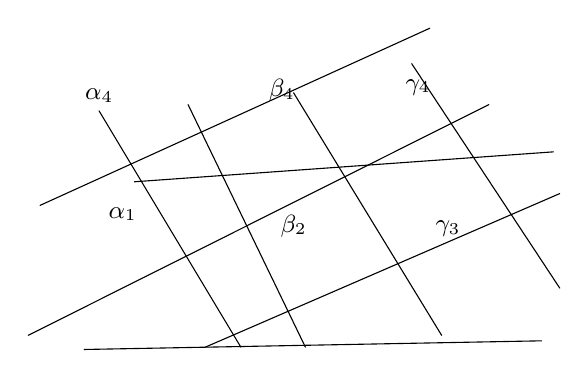
\begin{tikzpicture}[x=1mm,y=1mm,line cap=round,line join=round,font=\scriptsize]
\draw (31.5,-16.5) -- (49.5,-46.5);
\draw (42.8,-15.7) -- (57.7,-46.5);
\draw (56.2,-14.2) -- (75,-45);
\draw (71.2,-10.5) -- (90,-39);
\draw (24,-28.5) -- (73.5,-6);
\draw (22.5,-45) -- (81,-15.7);
\draw (45,-46.5) -- (90,-27);
\draw (36,-25.5) -- (89.2,-21.7);
\draw (29.6,-46.8) -- (87.7,-45.7);
\node[inner sep=1pt] at (31.5,-14.6) {\small $\alpha_4$};
\node[inner sep=1pt] at (54.7,-13.9) {\small $\beta_4$};
\node[inner sep=1pt] at (72,-13.5) {\small $\gamma_4$};
\node[inner sep=1pt] at (34.5,-29.6) {\small $\alpha_1$};
\node[inner sep=1pt] at (56.2,-31.1) {\small $\beta_2$};
\node[inner sep=1pt] at (75.8,-31.5) {\small $\gamma_3$};
\end{tikzpicture}
\end{document}
